\section{Introduction}
\subsection{Motivation and Logistics}
QFT is at the center of HEP, CMP, Soft matter/stat mech. Historically from HEP, but now useful everywhere. All the fields have their own insights, and their own answer into the question; why QFT?
\begin{itemize}
    \item HEP: Unique way to combine quantum physics with Lorentz invariance/SR; need it to describe the fundamental properties of the universe. This perspective is nicely emphasized in Weinberg. This was developed in parallel with experiments in particle physics, culminating in the standard model of particle physics, one of the most precise scientific theories that we have.
    \item CM: QFTs are an efficient way to parametrize many degrees of freedom, i.e. that may appear in many-body physics. An interesting notion here is then Effective Field Theories - in CM we aren't interested in the fundamental particles, generally; we know the microscopics of the system and can look at the emergent properties of a system. We can study EFTs that might be different from those that govern fundamental particles, that describe the system accurately at low-energy scales.
    \item Stat-mech: Field theories and QFT methods are very useful in classical contexts! As an example, in water, at a phase transition point between liquid and gas the system is described by a conformal field theory/CFT. In this context, we replace quantum fluctuations with thermal ones (statistical field theory). The idea of the renormalization group comes in, and coarse graining can give rise to universality.
    \begin{figure}[htbp]
        \centering
        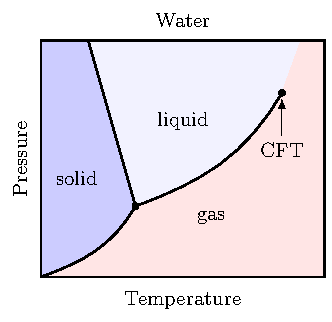
\includegraphics{Lectures/Figures/PT_diagram.pdf}
        \caption{Phase diagram of water. At the critical point, the system is described by a conformal field theory/CFT.}
        \label{fig:waterphase}
    \end{figure}
\end{itemize}

In this course we'll try to take a holistic perspective of QFT. The textbook is Srednicki - it's maybe not the best QFT textbook; it doesn't give good insights (come to lecture for that), but takes you through the details and developing techniques. Grade from weekly problem sets, assigned on Thursday and due the next Thursday.

\subsection{Review of Classical and Quantum Mechanics}
It will be useful to review the quantum simple harmonic oscillator as the simplest QFT is simply a collection of QSHOs.

\subsubsection*{Classical SHO - Variational Method}
Let's start with the classical SHO. Consider a (classical) point particle in a potential $V(x)$. 
\begin{figure}[htbp]
    \centering
    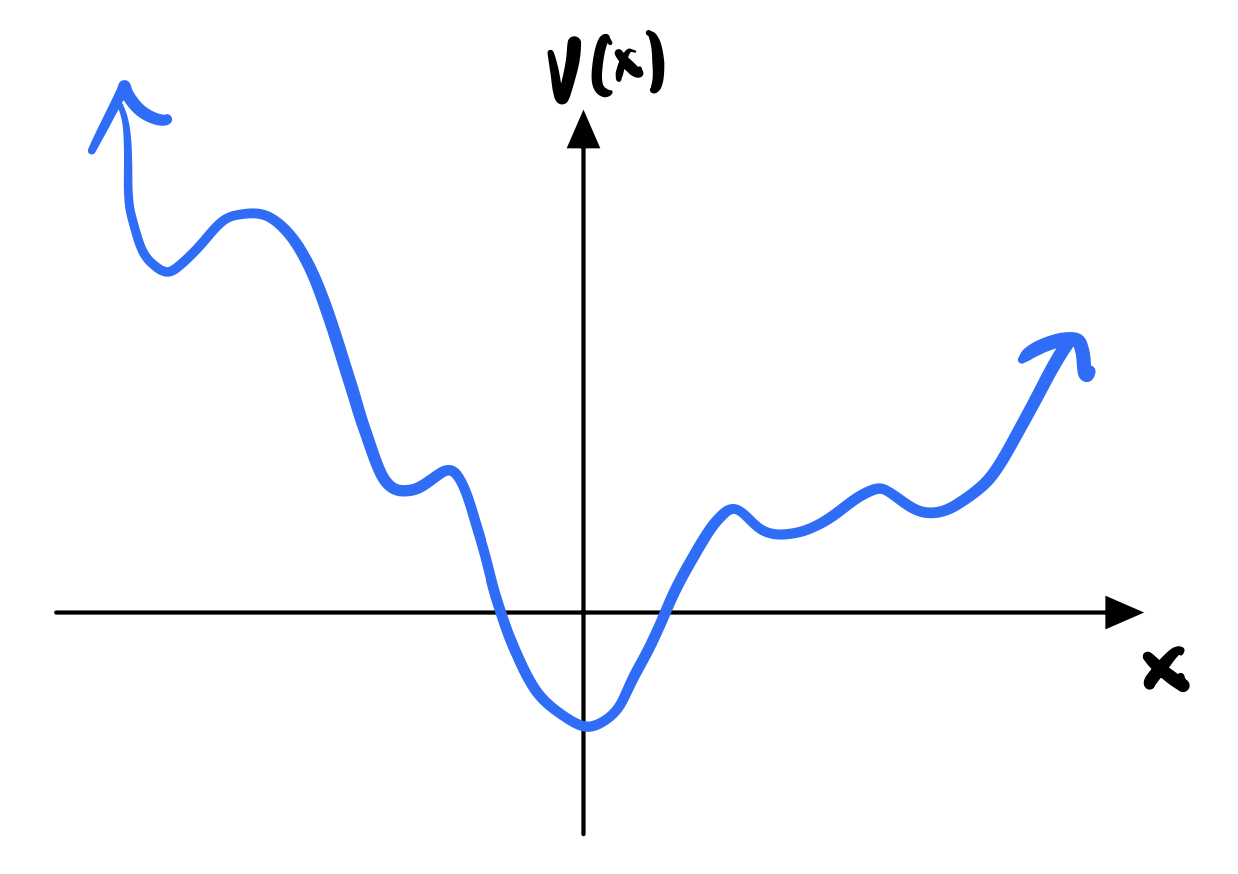
\includegraphics[scale=0.4]{Lectures/Figures/arbitrary_potential.png}
    \caption{Sketch of an arbitrary 1-D potential $V(x)$.}
    \label{fig:arbitrary_potential}
\end{figure}
Its dynamics is described by the action:
\begin{equation}
    S[x(t)] = \int dt \frac{1}{2}m\dot{x}(t) - V(x(t))
\end{equation}
where the first term is the kinetic energy and the second term is the potential energy.

To get the equation of motion from the action approach, we look for the trajectory $x(t)$ that extremizes the action (which is a \emph{functional}, as it depends on a function $x(t)$) $S[x(t)]$. We use a variational approach to find the extremizing trajectory. Under an arbitrary $\delta x(t)$ (to the true path $x(t)$), we must have $\delta S = 0$. Let us look at the variation, to linear order:
\begin{equation}
    0 = \delta S = \int dt m \dot{x}\dot{\delta x} - V'(x(t))\delta x
\end{equation}
Now, integrating by parts, we have:
\begin{equation}
    \int dt \dot{x}\dot{\delta x} = \left. \partial_t(\dot{x}\delta x) \right|_{-\infty}^\infty - \int dt \ddot{x}\delta x
\end{equation}
where the first term is a total derivative, which we take to be zero assuming the variation dies off at the infinite past and future. We then obtain:
\begin{equation}
    0 = \delta S = -\int dt \delta x(t)\left[m\ddot{x}(t) + V'(x(t))\right]
\end{equation}
Since this must vnaish for all variations $\delta x$, we obtain the equation of motion:
\begin{equation}
    \boxed{m\ddot{x}(t) + V'(x) = 0}.
\end{equation}

This is a nonlinear ODE, and difficult to solve; however when the potential is quadratic:
\begin{equation}
    V(x) = \frac{1}{2}kx^2
\end{equation}
\begin{figure}[htbp]
    \centering
    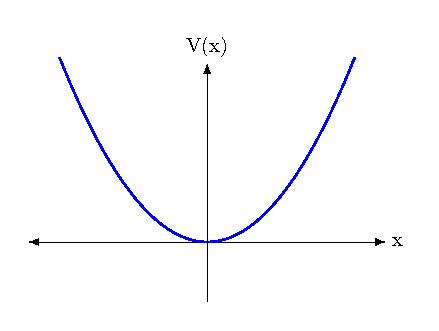
\includegraphics[]{Lectures/Figures/quad_potential.pdf}
    \caption{A quadratic potential $V(x) = \frac{1}{2}kx^2$.}
    \label{fig:quad_potential}
\end{figure}
it becomes linear and we can solve it! In this case, we have:
\begin{equation}
    0 = m\ddot{x} + kx
\end{equation}
The general solution is:
\begin{equation}
    x(t) = Ae^{i\omega_0t} + Be^{-i\omega_0t}
\end{equation}
where we have introduced the characteristic frequency $\omega_0 = \sqrt{k/m}$. $A, B$ are integration constants fixed by the initial conditions. Since we want $x(t) \in \RR$ for all $t$, this enforces $B = A^*$. 

\subsubsection*{Classical SHO - Hamiltonian Formalism}
We solve the same problem, but in the Hamiltonian formalism. We identify the conjugate momentum:
\begin{equation}
    p = \frac{\delta S}{\delta \dot{x}} = m\dot{x}
\end{equation}
And the Hamiltonian is given by:
\begin{equation}
    H = \dot{x}p - L = \frac{p^2}{m} - \frac{p^2}{2m} + V = \frac{p^2}{2m} + \frac{1}{2}kx^2
\end{equation}
and can be viewed as the generator of time translations. To obtain the EOM from the Hamiltonian, we consider the Poisson brackets:
\begin{subequations}
    \begin{align}
    \dot{x} &= \{x, H\}_{PB} \\
    \dot{p} &= \{p, H\}_{PB}
    \end{align}
\end{subequations}
Where $\{\}_{PB}$ denotes the Poisson bracket:
\begin{equation}
    \{f(x, p), g(x, p)\}_{PB} = \partial_x f \partial_p g - \partial_p f \partial_x g
\end{equation}
So the EOM become:
\begin{subequations}
    \begin{align}
        \dot{x} &= \partial_p H = \frac{p}{m} \\
        \dot{p} &= -\partial_x H = -kx
    \end{align}
\end{subequations}

From which we obtain:
\begin{equation}
    \dot{p} = m\ddot{x} = -kx
\end{equation}
which is precisely hte same equation we had previously.

A comment; the conjugate coordinate momentum pair satisfy:
\begin{equation}
    \{x, p\}_{PB} = 1.
\end{equation}

\subsection{The Quantum SHO}
In canonical quantization, one starts from the coordinates in phase space (in this case, $x$ and $p$) and then promotes them to quantum-mechanical operators satisfying canonical commutation relations:
\begin{equation}
    \{x, p\}_{PB} \to [\hat{x}, \hat{p}] = i\hbar
\end{equation}
where $\hbar$ is a constant with dimensions - by appropriate choice of units we can set it to 1, which we do for the remainder of this course. Thus, instead of measuring momentum in kg m/s, we will measure it in $\hbar$/m to make the commutator dimensionless.

$H$ is also now an operator; it has the same expression as before, but now involves $\hat{x}, \hat{p}$:
\begin{equation}
    \hat{H} = \frac{\hat{p}^2}{2m} + \frac{1}{2}k\hat{x}^2.
\end{equation}
$\hat{H}$ acts on states $\ket{\psi}$ of a Hilbert space. The dynamics are governed by the Schrodinger equation:
\begin{equation}
    i\partial_t \ket{\psi} = \hat{H}\ket{\psi}
\end{equation}
Acting on this equation with $\bra{x}$ a position eigenstate, we obtain the Scrodinger equation in position space:
\begin{equation}
    i\partial_t \psi(t, x) = -\frac{1}{2m}\partial_x^2\psi(t, x) + \frac{1}{2}kx^2\psi(t, x).
\end{equation}
where $\psi(t, x) \coloneqq \braket{x}{\psi}$ and we recall that $\hat{p} \to -i\partial_x$ when acting in position space (this can be derived from the canonical commutation relations).

This is a partial differential equation; in general, this is not trivial to solve (though we may of course put it on a computer and see the time evolution for arbitrary initial conditions). Instead of solving it fully generally, we look for stationary solutions:
\begin{equation}
    \psi(x, t) = e^{-iEt}\psi(x)
\end{equation}
We then obtain an ODE, which is slightly easier to work with:
\begin{equation}
    E\psi(x) = -\frac{1}{2m}\partial_x^2\psi(x) + \frac{1}{2}kx^2\psi(x).
\end{equation}
We would like for the solutions to be normalizable such that we are able to normalize $\psi(x)$ and interpret $\abs{\psi(x)}^2$ as a spatial probability distribution. Mathematically, this is the condition:
\begin{equation}
    \int dx \abs{\psi(x)}^2 < \infty.
\end{equation}
Although in the classical SHO we had an infinite, continuous set of solutions, the normalization condition interestingly reduces the set of solutions to a discrete (though still infinite) set. In this sense we have \emph{quantized} the SHO. We can label this discrete set of solutions as $\ket{n}$ for $n \in \NN$:
\begin{equation}
    \hat{H}\ket{n} = E_n\ket{n}.
\end{equation}

Let us review how to obtain the spectrum of the QSHO. We do this by diagonalizing $\hat{H}$, which we do via the method of raising and lowering operators, which are defined as linear combinations of $\hat{x}, \hat{p}$:
\begin{equation}
    \hat{a} = \frac{1}{\sqrt{2}}\left[\sqrt{m\omega_0}\hat{x} + i\frac{1}{\sqrt{m\omega_0}}\hat{p}\right]
\end{equation}
\begin{equation}
    \hat{a}^\dagger = \frac{1}{\sqrt{2}}\left[\sqrt{m\omega_0}\hat{x} - i\frac{1}{\sqrt{m\omega_0}}\hat{p}\right]
\end{equation}
The coefficients are chosen such that:
\begin{equation}
    [\hat{a}, \hat{a}^\dagger] = 1
\end{equation}
and such that:
\begin{equation}
    \hat{H} = \omega_0(\hat{a}^\dagger \hat{a} + \frac{1}{2})
\end{equation}
Defining $N \coloneqq \hat{a}^\dagger a$, the eigenstates are discrete; let $\ket{n}$ be the eigenstates of $\hat{N}$:
\begin{equation}
    \hat{N}\ket{n} = n\ket{n}.
\end{equation}
we show that $n \in \NN$. This follows as:
\begin{equation}\label{eq:lowering}
    \hat{N}\hat{a}\ket{n} = \hat{a}^\dagger \hat{a}\hat{a}\ket{n} = ([\hat{a}^\dagger, \hat{a}] - \hat{a}\hat{a}^\dagger)\hat{a}\ket{n} = -\hat{a}\ket{n} + \hat{a}\hat{a}^\dagger \hat{a}\ket{n} = (n-1)\hat{a}\ket{n}
\end{equation}
so $\hat{a}$ lowers the eigenvalue of $\hat{N}$ by one. In order for the spectrum to be bounded, we require a state annihilated by $\hat{a}$, i.e. that which $\hat{a}\ket{0} = 0$ (else there is no lower bound to the spectrum). We then note that:
\begin{equation}
    \hat{N}\ket{0} = \hat{a}^\dagger\hat{a}\ket{0} = 0 = 0\ket{0}
\end{equation}
thus this is an eigenstate (the ground state) of $\hat{H}$ with eigenvalue $\omega_0/2$. The rest of the spectrum can be built using $\hat{a}^\dagger$s. Via a similar argument to Eq. \eqref{eq:lowering}, it can be shown that $\hat{a}^\dagger$ increases the eigenvalue of $\hat{N}$ by one, and thus the eigenstates are:
\begin{equation}
    \ket{n} = \frac{(\hat{a}^\dagger)^n}{\sqrt{n!}}\ket{0}
\end{equation}
where $\braket{n}{n'} = \delta_{nn'}$, $\hat{N}\ket{n} = n\ket{n}$, and $\hat{H}\ket{n} = \omega_0(n + \frac{1}{2})\ket{n}$. Thus the spectrum is:
\begin{equation}
    \boxed{E_n = \omega_0(n + \frac{1}{2})}.
\end{equation}

This QSHO will be the building block from which we will construct quantum field theories.

\subsection{Free Scalar QFT}
Consider a SHO on every site of a $M$-site lattice:
\begin{figure}[htbp]
    \centering
    
\includegraphics[scale=0.4]{Lectures/Figures/qsho_chain.png}
    \caption{We begin to construct the simplest QFT, the free scalar QFT, by placing non-interacting quantum SHOs on sites of a lattice.}
    \label{fig:qsho_chain}
\end{figure}
The action is then simply the $M$-fold sum of our previous action
\begin{equation}
    S = m\sum_{j=1}^M\int dt \frac{1}{2}\dot{x}_j(t) - \frac{1}{2}\omega_0^2x_j(t) = \sum_{j=1}^M\int dt \frac{1}{2}\dot{\phi}_j^2(t) - \frac{1}{2}\omega_0^2\phi_j(t)
\end{equation}
where we have defined $\phi_j = \sqrt{m}x_j$. This is a quantum many-body system, but the solution to this is already known! It will simply be $M$ copies of the previous single-body system. Eigenstates are labelled by a collection of occupation numbers $\set{n_j}$, where:
\begin{equation}
    \ket{\set{n_j}} = \ket{n_1, n_2, \ldots, n_M}
\end{equation}
and the energy eigenvalues is just the sum of the individual energies:
\begin{equation}
    \hat{H}\ket{\set{n_j}} = \sum_j E_j \ket{\set{n_j}} = \sum_j \omega_0(n_j + \frac{1}{2})\ket{\set{n_j}}.
\end{equation}

\subsubsection*{Adding interactions}
This will become more interesting if we couple the SHOs, for example with nearest neighbour couplings. We add a term to the action:
\begin{equation}
    S = \sum_{j=1}^M \int dt \frac{1}{2}\dot{\phi_j}^2 - \frac{1}{2}\omega_0\phi_j^2 - \frac{1}{2}\frac{c^2}{\delta^2}(\phi_j - \phi_{j-1})^2
\end{equation}
The last term represents an energy penalty to the positions of neighbouring oscillators not being aligned. 

\begin{figure}[htbp]
    \centering
    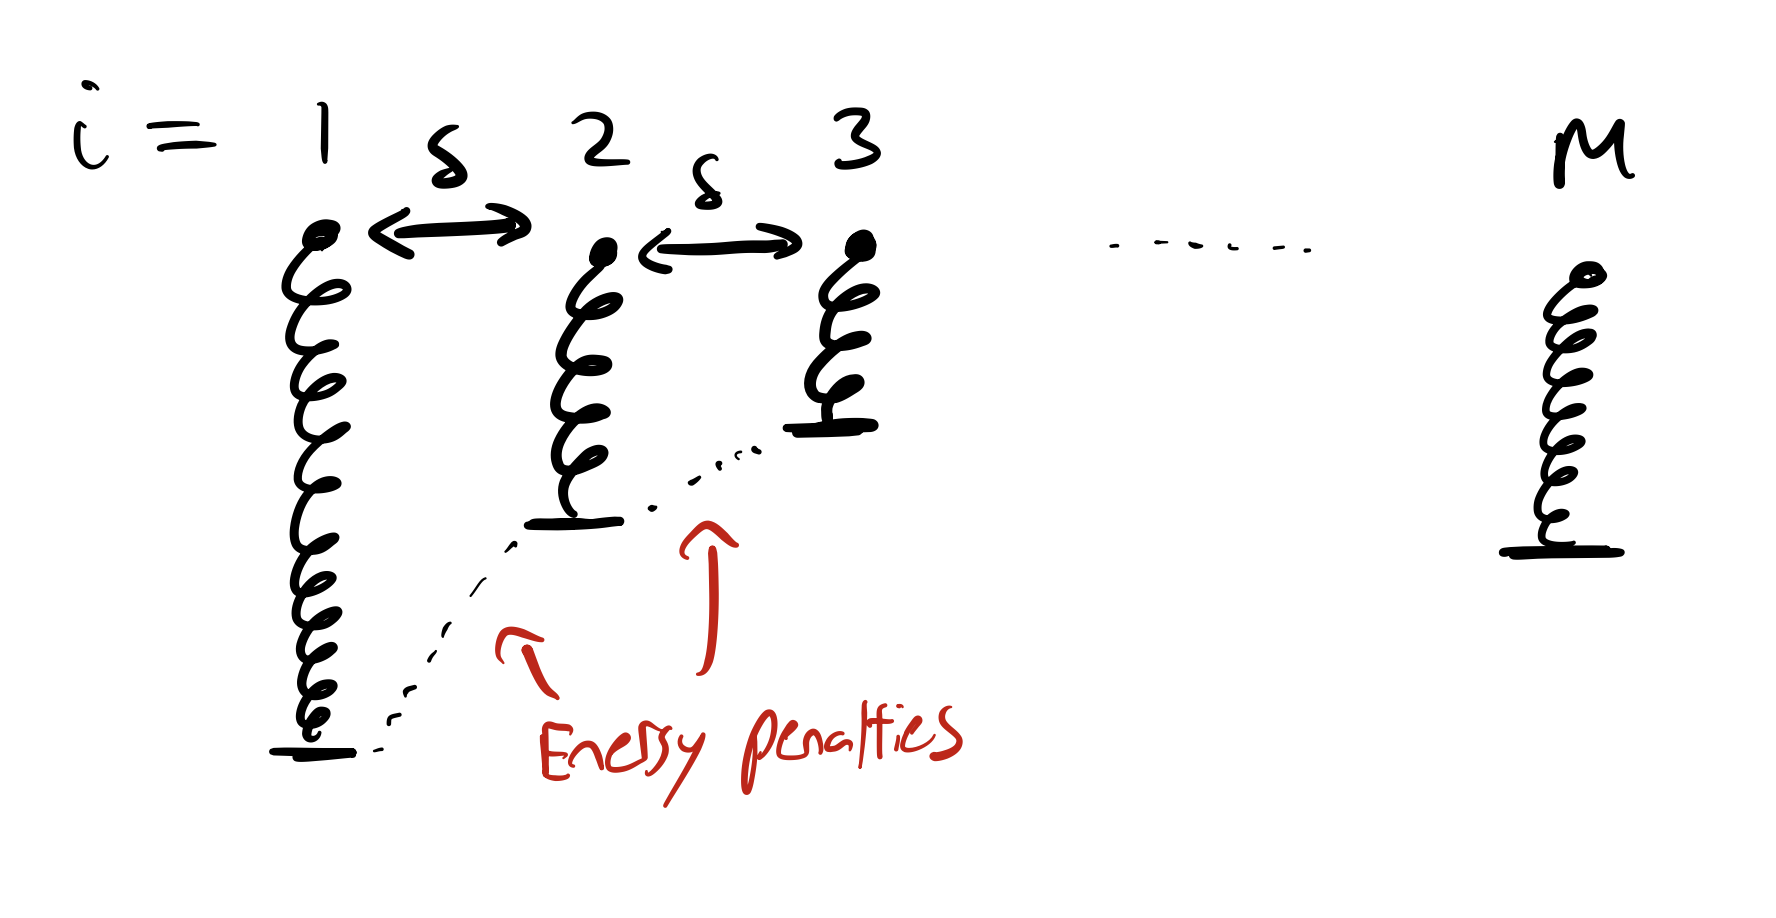
\includegraphics[scale=0.4]{Lectures/Figures/coupled_qsho_chain.png}
    \caption{We introduce couplings between QSHOs by imposing an energy penalty when neighbouring oscillators are misaligned. The relevant length scale of the interaction is given by the lattice spacing $\delta$.}
    \label{fig:coupled_qsho_chain}
\end{figure}

$\delta$ is the spacing between lattice sites and $c$ has the dimensions of velocity. The term must have units of $\frac{1}{t^2}$, and we see that $\frac{c^2}{\delta^2}$ indeed has this.

This turns out to be a much richer system! The action/Hamiltonian is not diagonal in the $i$ label. The trick is to do a change of basis, via a Fourier transform:
\begin{equation}
    \tilde{\phi}_k = \frac{1}{\sqrt{M}}\sum_{j=1}^Me^{-i\delta k j}\phi_j
\end{equation}
which we will show can be inverted:
\begin{equation}
    \phi_j = \frac{1}{\sqrt{M}}\sum_{k=1}^Me^{i\delta k j}\tilde{\phi}_k
\end{equation}
and $k \in \{-\frac{M}{2} + 1, \ldots, -1, 0, 1, \ldots, \frac{M}{2}\} \cdot \frac{2\pi}{L}$. We will then show that:
\begin{equation}
    S = \sum_k \int dt \frac{1}{2}\abs{\tilde{\phi}_k}^2 - \frac{1}{2}\omega_0^2\abs{\tilde{\phi}_k}^2 - \frac{c^2}{\delta^2}(1 - \cos(k\delta))\abs{\tilde{\phi}_k}^2.
\end{equation}
We then notice that the $\tilde{\phi}_k$s don't talk to each other/are decoupled! We are back to having decoupled SQHOs, just in a different basis. This immediately gives the spectrum.